\section{Moments}\label{s: moments}
Having defined the techniques required to compute fractional derivatives, we now turn to their application to the Moment Generating Function (MGF). Before proceeding, we will briefly review some key concepts related to statistical moments.
\subsection{Moments}
\begin{definition}
    Let \(X\) be a random variable.
    The \(\alpha\)-th moment of a \(X\) is defined as:
   \[
\mathbb{E}[X^\alpha] = 
\begin{cases} 
\int_{-\infty}^{\infty} (x - c)^\alpha f_X(x) \, dx & \text{if } X \text{ is continuous,} \\ 
\sum_{i} (x_i - c_ i)^\alpha f_X(x_i) & \text{if } X \text{ is discrete.} 
\end{cases}
\] with, in the context of this paper \(\alpha \in \mathbb{R}\). Here \(f_X(x)\) is the probability density function if \(X\) is a continuous random variable, and the probability mass function if \(X\) is a discrete random variable.
\end{definition}

If \(c = \mu_x\), the first moment of \(f(x)\), then our higher moments are called central moments. In the context of this research, we will focus on the case \(c = 0\), corresponding to raw moments of a random variable \(X\). This choice has been made as the Moment Generating Function, which we will soon define, only computes raw moments of higher order. A moment of order \(n\) is said to exist, if \(\mathbb{E}[X^n] < \infty\).

The following proposition is rather standard and well known. Yet, since we will be working with a lot of fractional moments which replace non-existing integer moments, it does not hurt to reiterate these properties.

\begin{proposition}\label{p: moments_1}
    Let \(X\) be a random variable. Then:
    \begin{enumerate}[(i)]
        \item If \(\mathbb{E}[X^n]\) does not exist, then neither does \(\mathbb{E}[X^k]\), for \( n \leq k\).
    
    \item If \(\mathbb{E}[X^k]\) does exist, then all its lower-order moments, \(\mathbb{E}[X^n]\), for \(n \leq k\). Also exists.
\end{enumerate}
\end{proposition}
The proof is rather straightforward and can be found in Appendix \ref{s:app_B}.


\subsubsection{Moments of negative order}
Since the MGF can be extended to negative orders, we briefly examine how to compute raw moments of negative order using traditional methods. This will allow us to compare results between the two different methods. What is more, as mentioned in section \ref{s:intro}, in specific cases, moments of negative order can be computed to obtain statistics such as the Sharpe Ratio. Thus, it is useful to understand how to compute moments of such orders. We will consider the continuous case:
\[\mathbb{E}[X^{-n}] = \int_{-\infty}^{\infty} x^{-n} f_X(x) dx = \int_{-\infty}^{\infty} \left(\frac{1}{x}\right)^n f_X(x) dx.\] We can immediately observe a rather obvious problem. This integral is undefined at \(x = 0\) and diverges in a neighbourhood around zero. \cite{khuri2002} have stated the following corollary for the existence of a moment with negative first order:
\begin{corollary}
    If \(f_X(x)\) is a continuous pdf defined on \((-\infty, \infty)\), and if \[\lim_{x \to 0} \frac{f_X(x)}{|x|^\alpha} < \infty\] for \(\alpha > 0\), then \[\mathbb{E}[X^{-1}] \text{ exists}.\]
\end{corollary}

Most common distribution functions do not adhere to this corollary, however, the Gamma function does:

\begin{example}\label{e: negative}
    Let \(f_X(x) \sim \Gamma(\alpha, \lambda) =\) 
    \[\frac{x^{\alpha -1} e^{-\lambda x} \lambda^\alpha} {\Gamma(\alpha)}.\] This PDF is defined on \((0, \infty)\). So the function is not defined on \(\mathbb{R}\). This, however, is not a problem, as we can just evaluate the right limit. Since the Gamma function already uses \(\alpha\) as a parameter, we will evaluate \(\frac{f_X(x)}{|x|^\beta}, \beta > 0\):
    \[\lim_{x \to 0_+} \frac{f_X(x)}{|x|^\beta} = \lim_{x \to 0_+} \frac{x^{\alpha -1 - \beta} e^{-\lambda x} \lambda^\alpha} {\Gamma(\alpha)} = \lim_{x \to 0_+} \frac{x^{\alpha -(1 + \beta)} e^{-\lambda x} \lambda^\alpha} {\Gamma(\alpha)} .\] Thus for \(\alpha \geq \beta + 1, \lim_{x \to 0_+} \frac{f_X(x)}{|x|^\beta} < \infty\). Therefore, the first negative moment of the Gamma distribution should exist.

    We will compute the first negative moment: 
    \[ \mathbb{E}[X^{-1}] = \int_{0}^{\infty} x^{-1} \frac{x^{\alpha -1} e^{-\lambda x} \lambda^\alpha} {\Gamma(\alpha)} dx = \frac{\lambda^\alpha}{\Gamma(\alpha)} \int_{0}^{\infty} x^{\alpha - 2} e^{-\lambda x} dx\]
    Using the substitution \( u = \lambda x, \frac{du}{dx} = \lambda, dx = \frac{du}{\lambda}\), we get:
    \[ = \frac{\lambda^\alpha}{\Gamma(\alpha)} \int_{0}^{\infty}\left(\frac{u}{\lambda}\right)^{\alpha -2} e^{-u} du = \frac{\lambda^\alpha}{\Gamma(\alpha) \lambda^{\alpha-1}} \int_{0}^{\infty}(\frac{u}{\lambda})^{\alpha -2} e^{-u} du.\] This integral is equal to \(\Gamma(\alpha - 1)\) (See Appendix \ref{s:appendices}). So we get: 
    \[\mathbb{E}[X^{-1}] = \frac{\lambda^\alpha \Gamma(\alpha - 1) }{\Gamma(\alpha) \lambda^{\alpha-1}} = \frac{\lambda \Gamma(\alpha - 1)}{(\alpha -1)\Gamma(\alpha - 1)} = \frac{\lambda}{(\alpha -1)}.\] Thus, for \(\alpha \neq 1, \mathbb{E}[X^{-1}] = \frac{\lambda}{(\alpha -1)}\). Fortunately, this is always the case, since we had just derived that the integral only converges when \(\alpha \geq \beta + 1, \text{ with } \beta > 0\). In other words, \(\alpha > 1\). So this holds.
\end{example}
\subsection{The Moment Generating Function}
We now formally introduce the Moment Generating Function, one of the most significant subjects of this thesis.
\begin{definition}
    The Moment Generating Function (MGF) of a variable \(X\), is defined as
    \[M_X(t) = \mathbb{E}[e^{tX}]\] provided that \(\mathbb{E}[e^{tX}] < \infty\), for all  \( t \in (- h, h)\), which contains 0, for some \(h > 0\).
\end{definition}

\begin{remark}
    Deriving the expression \(M_X(t) = \mathbb{E}[e^{tX}]\) is typically straightforward. Generally, it simply requires a handful of steps of analytic evaluation. This procedure is not that interesting nor relevant to this research. We provide a single explicit example on how to compute the Moment Generating Function for a specific distribution below. And for later cases, when we make use of an expression of the Moment Generating Function, we will simply refer to the distribution table in Appendix \ref{t: MGF_Appendix}.
\end{remark}

\begin{example}
    Let \(f_X(x) \sim \Gamma(\alpha, \lambda)\) be the Gamma distribution with PDF:
     \[
     f_X(x) = \frac{x^{\alpha -1} e^{-\lambda x} \lambda^\alpha}{\Gamma(\alpha)}.
     \]
     Let \( t < \lambda\) (in any other case, the integral diverges).The moment generating function \(M_X(t)\) is given by:
     \[
     M_X(t) = \int_{0}^{\infty} e^{tx} f_X(x) \, dx = \frac{\lambda^\alpha}{\Gamma(\alpha)} \int_{0}^{\infty} x^{\alpha -1} e^{(t - \lambda) x} \, dx.
     \]
     We make use of the substitution \(u = -(t - \lambda)x\), \(\frac{du}{dx} = (\lambda - t)\), \(dx = \frac{du}{(\lambda - t)}\), so:
     \[
     = \frac{\lambda^\alpha}{\Gamma(\alpha)} \int_{0}^{\infty} \left(\frac{u}{\lambda - t}\right)^{\alpha -1} e^{-u} \frac{du}{\lambda - t} = \frac{\lambda^\alpha}{\Gamma(\alpha) (\lambda - t)^\alpha} \int_{0}^{\infty} u^{\alpha -1} e^{-u} \, du.
     \] This integral is just the definition of the Gamma Function, \(\Gamma(\alpha)\), so we obtain:
     \[ = \frac{\lambda^\alpha \Gamma(\alpha)}{\Gamma(\alpha) (\lambda - t)^\alpha} = \left(\frac{\lambda}{\lambda - t}\right)^\alpha = M_X(t)\]
 \end{example}
 
We will state the theorem which makes the MGF so useful. This theorem allows us to compute moments of higher order by taking derivatives of the given order instead of integrals.
\begin{theorem}\label{t: mgf}
    If \(M_X(t)\) exists on some interval \((-h, h)\), as defined before, we have that:
    \[ \mathbb{E}[X^n] = M_X^{(n)}(0), \text{ for } n \in \mathbb{N}\]
\end{theorem}

\begin{proof}
    The proof is important and fairly straightforward, thus it will be shown directly:
    \[M_X^{(n)}(t) = \frac{d^n}{dt^n} \int_{-\infty}^{\infty} e^{tx} f_X(x) dx = \int_{-\infty}^{\infty} \frac{d^n}{dt^n} e^{tx} f_X(x) dx\] (We can interchange differentiation and integration since all partial derivatives of \(e^{tx} f(x)\) are continuous and the absolute value of the integral converges, as we assume the \(n\)-th moment exists, see Appendix \ref{s:appendices}).
    \[ = \int_{-\infty}^{\infty} x^n e^{tx} f_X(x) dx, \text{evaluating at } t = 0: = \int_{-\infty}^{\infty} x^n e^{0x} f_X(x) dx\]
    \[ = \int_{-\infty}^{\infty} x^n f_X(x) dx = \mathbb{E}[X^n]\]
    The proof for the case that \(f_X(x)\) is discrete is very similar. In that case, one would have to change the order of the derivative and summation, which has also been justified in Appendix \ref{s:appendices}.
\end{proof}


We introduce the following properties for the Moment Generating Function \(M_X(t)\):
\begin{proposition}\label{p: moments}
    For \(X, Y\) random variables, we have that:
    \begin{enumerate}[(i)]
        \item \(M_X^{(0)}(t) = \mathbb{E}[e^{0X}] = 1\). This property can be used to confirm that a given function is a valid probability density function (i.e., integrates to one).
        \item Location scale-transform. Assuming \(M_X(t)\) exists, for constant \(\mu, \sigma\), we have that: 
        \[M_{\mu + \sigma X}(t) = e^{\mu t} \cdot M_X(\sigma t)\]
        \item If \(X \perp Y\), then \(M_{X+Y}(t) = M_X(t)\cdot M_Y(t)\).
    \end{enumerate}
\end{proposition}

The proofs of the latter can be found in Appendix \ref{s:app_B}.

There are several additional topics closely related to the MGF, including Fourier transforms, Laplace transforms, Wick rotations, and characteristic functions. While these subjects are relevant to the theoretical foundation of the MGF , they fall outside the scope of this paper and will therefore not be discussed. Readers interested in exploring these concepts further may find \cite{kolmogorov1999} to be a valuable resource.

\subsubsection{Computing negative moments using the Moment Generating Function}
We have seen that under specific conditions, it is possible to compute negative, or so called inverse moments of distribution functions. This technique can also be applied to the moment generating function. In the 20-th century, \cite{cressie1981} have published the following remarkable theorem:

\begin{theorem}\label{t: negative}
    Assuming the negative \(n\)-th raw moment exists, the negative \(n\)-th raw moment can be computed as follows: 
    \[\mathbb{E}[X^{-n}] = \frac{1}{\Gamma(n)} \int_{0}^{\infty} t^{n- 1} M_X(-t) dt\] where \(n\) is a positive integer.
\end{theorem}
The proof of this Theorem can be found in Appendix \ref{s:app_B}.

Since this is an extension on the regular functions of the MGF, this technique is of interest of this paper. Thus, it will be shortly be discussed. Let us again compute the first inverse moment of the Gamma distribution, but now by making use of the latter theorem for Moment Generating Functions!

\begin{example}
    Let \[f_X(x) \sim \Gamma(\alpha, \lambda) = 
    \frac{x^{\alpha -1} e^{-\lambda x} \lambda^\alpha} {\Gamma(\alpha)}, M_X(t) = \left(\frac{\lambda}{\lambda - t}\right)^\alpha\]
    \[\mathbb{E}[X^{-1}] = \frac{1}{\Gamma(1)} \int_{0}^{\infty} t^{( 1 - 1)} \left(\frac{\lambda}{\lambda - (-t)}\right)^\alpha dt =  \int_{0}^{\infty} \left(\frac{\lambda}{\lambda + t}\right)^\alpha dt\]
    \[ = \lambda^\alpha \int_{0}^{\infty} (\lambda + t)^{-\alpha} dt, \text{ Let } u = \lambda + t, \frac{du}{dt} = 1, dt = du:\]
    \[ \lambda^\alpha \int_{0}^{\infty} u^{-\alpha} du
    =  \lambda^\alpha \frac{u^{ 1-\alpha}}{1 -\alpha}\Big|_{0}^{\infty} = \lambda^\alpha \frac{(\lambda + t)^{1 -\alpha}}{1 -\alpha}\Big|_{0}^{\infty}\]
    \[= \lambda^\alpha\left( 0 - \frac{\lambda^{ 1 - \alpha}}{1 -\alpha}\right) = \frac{-\lambda}{ 1 - \alpha} = \frac{\lambda}{\alpha - 1}.\] Which corresponds with our result from example \ref{e: negative}.
\end{example}

\subsubsection{Extending the MGF to fractional order}
Now that we have introduced the definitions of the MGF and discussed some key properties, we will combine these with the techniques developed in section \ref{s:calculus}. Therefore, we can at last obtain moments of fractional order using the MGF.


To avoid confusion regarding what fractional derivative is being used in combination with the MGF, we will from now on, work with the following notation:
\begin{definition}\label{d: MGF}
    We define the MGF of order \(\alpha \in \mathbb{R}\) by \(\leftindex_{RL}{M}_X^{(\alpha)}, \leftindex_{CF}{M}_X^{(\alpha)}, \leftindex_{GL}{M}_X^{(\alpha)}\) for the MGF in combination with the Riemann-Liouville, Caputo-Fabrizio and Grünwald-Letnikov fractional derivative respectively.
\end{definition}
\begin{remark}
    The three properties mentioned in proposition \ref{p: moments} still hold for the MGF of fractional order. This is the case as the first property makes makes use of the derivative of order 0. Which has been defined to just be the original function itself as stated in the second property of proposition\ref{p: calculus}. The other two properties do not involve any derivatives of any order. Thus, they are generally applicable to the MGF, regardless of its order or kind of derivative.
\end{remark}

Before stating any results about the accuracy of these new MGF expressions, we first consider a numerical example to illustrate the interaction between fractional derivatives and the MGF. 

\begin{example}
    \begin{enumerate}[(i)]
        \item We let \(f_X(x) \sim Bernoulli(p)\), with \(\mathbb{P}(X = 1) = p\) and with associated MGF expression: \(M_X(t) = (1 - p) + p \cdot\exp(t)\), now we consider \[\leftindex_{CF}{M}_X^{(\frac{1}{2})} = \frac{1}{1 - \frac{1}{2}}  \int_{-h}^{t} \exp\left(\frac{\frac{-1}{2}}{1 - \frac{1}{2}}(t-s)\right) f'(s) ds.\] In this case, the domain of \(f(t) = (-\infty, \infty)\), so we let \(-h = -\infty\), and \(f'(s) = p\cdot \exp(s)\), thus we obtain:
        \[\leftindex_{CF}{M}_X^{(\frac{1}{2})} = 2  \int_{-\infty}^{t} \exp\left((s-t)\right) \cdot (p\cdot \exp(s)) ds.\]
        \[= 2p \cdot exp(-t) \int_{-\infty}^{t}\exp(2s) ds\] 
        \[= p\cdot exp(-t) \left(\exp(2s) \Big|_{-\infty}^{t}\right) = p\cdot \exp(t)\]
        Now, all that is left to do is set \(t = 0\) and we obtain that \(\leftindex_{CF}{M}_X^{(\frac{1}{2})} = p\).
        \item Computing \(\mathbb{E}[{X^{\frac{1}{2}}}]\) in the traditional fashion, we obtain: 
        \[\mathbb{E}[{X^{\frac{1}{2}}}] = \sum_x x^{\frac{1}{2}} \mathbb{P}(X = x) = 0^{\frac{1}{2}} \cdot \mathbb{P}(X = 0) + 1^{\frac{1}{2}} \cdot \mathbb{P}(X = 1)\]
        \[ = 0 \cdot(1 - p) + 1 \cdot p = p\]
    \end{enumerate}
    
\end{example}
It is amazing and maybe even somewhat surprising that both expressions obtain the same result. Indeed, this result is actually more of a coincidence. It is important to note that this agreement of results is coincidental and specific to the chosen distribution. Namely, all raw higher moments of a Bernoulli random variable are \(p\). If we had taken any other distribution in combination with a moment of fractional order, it becomes highly likely that the MGF returns a different value compared to the traditional method of computing moments. What is more, if we were to take \[\leftindex_{RL}{M}_X^{(\frac{1}{2})}  = \frac{d}{dt} \frac{1}{\sqrt{\pi}}  \int_{-h}^{t} (t - s)^{\frac{-1}{2}} f(s) ds\] we obtain an integral which may diverge based on the choice of \(-h\) . These observations lead to the following theorem.

\begin{theorem}\label{t: MGF_accurate}
     Consider the three MGF's as defined in definition \ref{d: MGF}. Assume \(\leftindex_{RL}{M}_X^{(\alpha)}\) and \(\leftindex_{GL}{M}_X^{(\alpha)}\) are well defined on some open interval \((-h, h)\), then the moment generating function expressions \(\leftindex_{RL}{M}_X^{(\alpha)}\) and \(\leftindex_{GL}{M}_X^{(\alpha)}\) accurately obtain moments of order \(\alpha \in \mathbb{R}\)
    
\end{theorem}
The proof can be found in Appendix \ref{s:app_B}.
Unfortunately, this result does not hold for \(\leftindex_{CF}{M}_X^{(\alpha)}\), which leads to the following theorem.

\begin{theorem}\label{t: MGF_inaccurate}
    Consider the three MGF's as defined in definition \ref{d: MGF}. Assume \(\leftindex_{CF}{M}_X^{(\alpha)}\) is well defined on some open interval \((-h, h)\), then the moment generating function expression \(\leftindex_{CF}{M}_X^{(\alpha)}\) inaccurately approximates moments of order \(\alpha \in \mathbb{R}\) with approximation error given by
    \[
\begin{cases} 
    \displaystyle \int_{-\infty}^{\infty} x^\alpha  f_X(x) dx -  \displaystyle \int_{-\infty}^{\infty}  \frac{x^{n+1} }{(1 - \beta)x + \beta} f_X(x) dx & \text{if } X \text{ is continuous,} \\ 
    \displaystyle \sum_{i} \left(x_i^\alpha -  \frac{x_i^{n+1} }{(1 - \beta)x_i + \beta}\right) f_X(x_i) & \text{if } X \text{ is discrete.} 
\end{cases}
\] with \(\alpha \in \mathbb{R}, \beta = \alpha - n \text{ and } n = \lfloor \alpha \rfloor.\)
    
\end{theorem}
The proof can be found in Appendix \ref{s:app_B}.

\begin{remark}
    In the case when \(\alpha \in \mathbb{N}\), we have that \(n = \alpha\), and thus \( \beta = 0\), therefore, \(\leftindex_{CF}{M}_X^{(\alpha)}\) is accurate for integer orders. This is an expected result, as the MGF for integer moments is accurate and from section \ref{s:calculus} we know that \(D_{CF}^{\alpha + \beta}f(x) = D_{CF}^\alpha(D_{CF}^\beta f(x))\), with \(\alpha \in \mathbb{N}, \beta \in [0, 1).\) In this case, let \(\beta = 0\). So we get \(D_{CF}^{\alpha + 0}f(x) = D_{CF}^{\alpha}f(x)\) which is just a regular derivative of integer order.
\end{remark}
\subsubsection{Analysing the error of the Caputo-Fabrizio MGF}
We now further inspect the error obtained in theorem \ref{t: MGF_inaccurate}. Note that in the following plots, we explicitly focus on the term \[ E(x, \alpha) = x^\alpha - \displaystyle \frac{x^{n+1} }{(1 - \beta)x + \beta}\] for simplicity. The expression we analyse, denoted \(E(x, \alpha)\) is not the same as the expression obtained in theorem\ref{t: MGF_inaccurate}. Yet, it is the part of the expression that involves the order \(\alpha\) and is thus of great interest. What is more, considering the result obtained in theorem \ref{t: MGF_inaccurate}, it is easy to see that \(\leftindex_{CF}{M}_X^{(\alpha)}\) is accurate \(\iff x^\alpha = \displaystyle \frac{x^{n+1} }{(1 - \beta)x + \beta}\). Thus, we consider the function \(E(x, \alpha)\), the function of their differences and analyse when this function is equal to 0. Errors of the Caputo-Fabrizio MGF as defined in theorem \ref{t: MGF_inaccurate} will be explicitly numerically computed in the following section of this paper, where we will consider a multitude random variables, with different distributions. Plotting this expression for different orders of \(\alpha\), we obtain the following figure:
\begin{figure}[H]
    \centering
    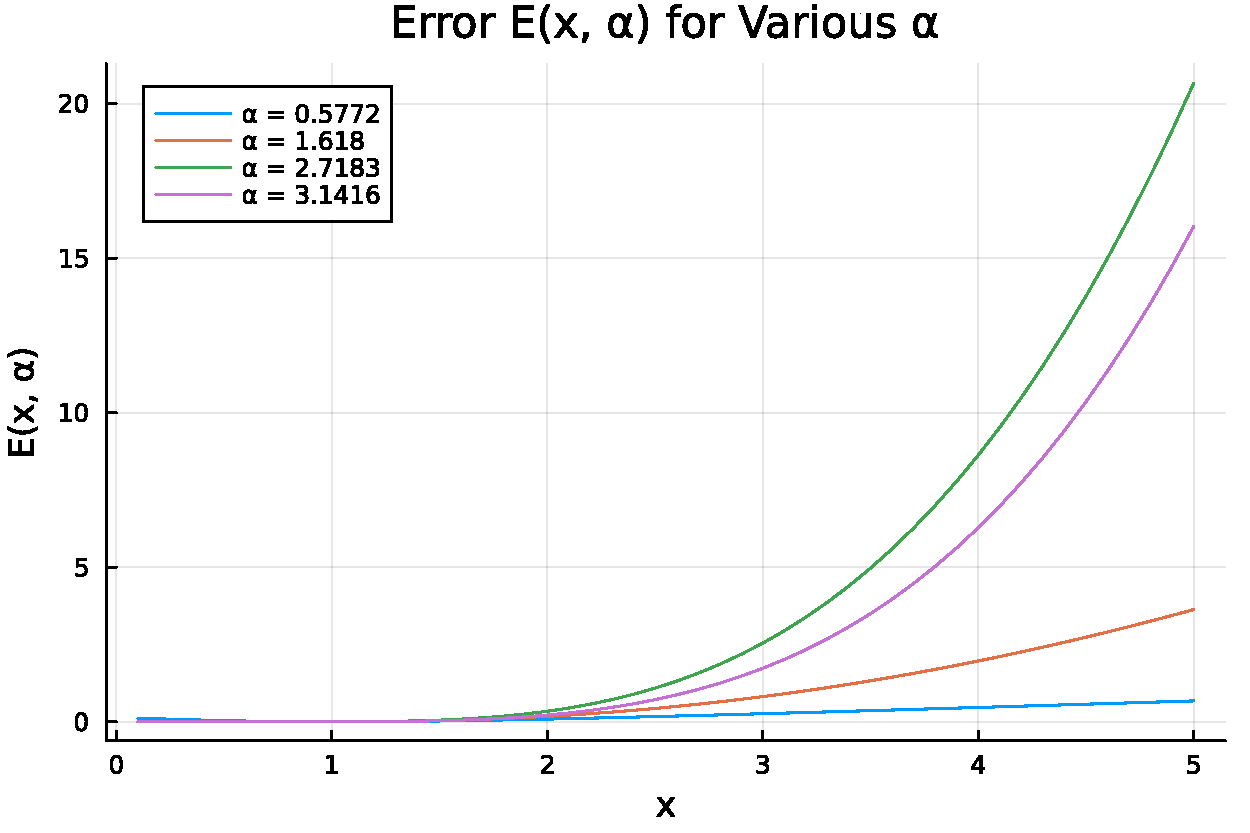
\includegraphics[width=0.8\textwidth]{figures/error_plot.pdf}
    \caption{Error of Caputo-Fabrizio MGF}
    \label{fig:error_MGF}
\end{figure}
It can be observed from the figure above that, in general for greater orders \(\alpha\), the error tends to increase. However, the greatest order of \(\alpha\) does not provide the greatest error. Instead it is the second greatest order of \(\alpha\) that does so. This may be explained by the fact that for values of \(\alpha\) in the middle of two integers, the value of \((1 - \beta)x + \beta\) will be the greatest. As a result, the fraction becomes small, so the error tends to increase.

This hypothesis is indeed confirmed in the following figure, which focuses on the growth rate of the error, for a fixed value of \(x\) and an increasing order \(\alpha\).

\begin{figure}[H]
    \centering
    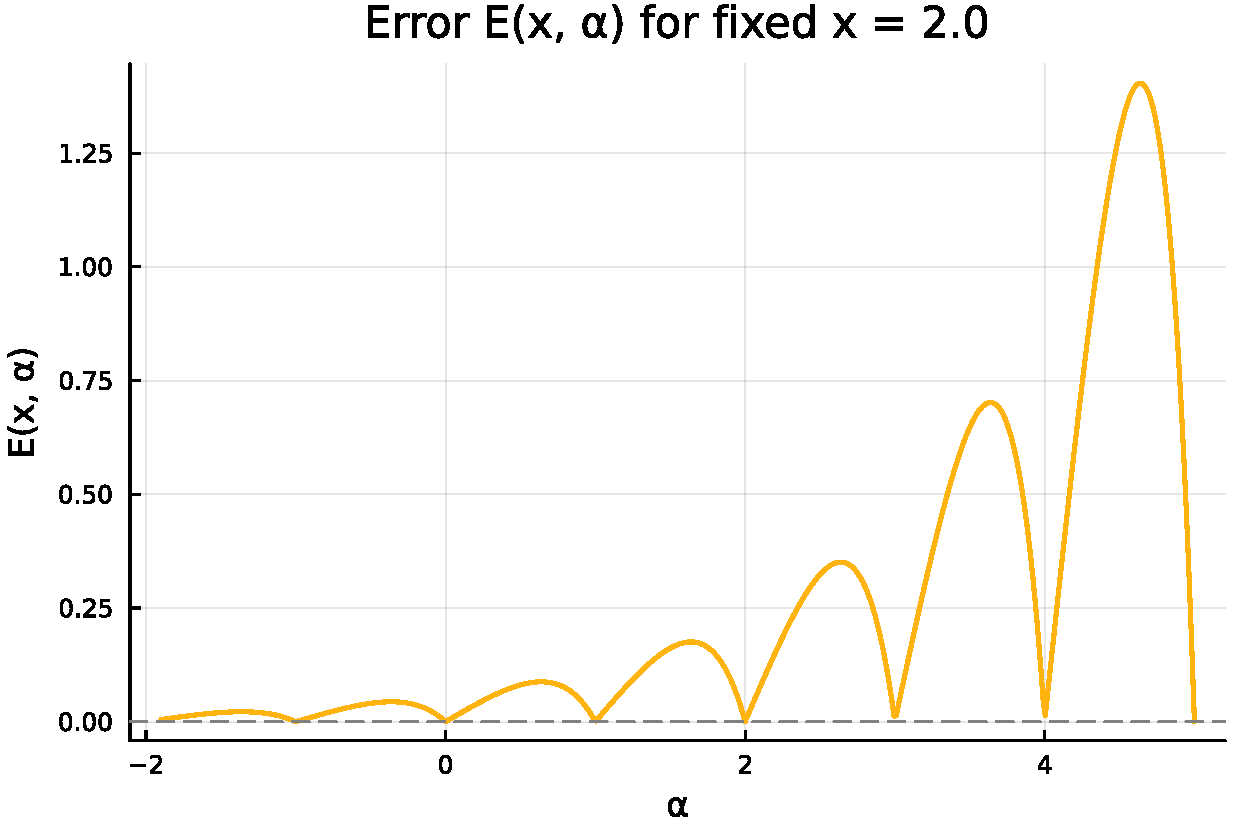
\includegraphics[width=0.8\textwidth]{figures/error_plot_fixed_x.pdf}
    \caption{Error of Caputo-Fabrizio MGF, for fixed x}
    \label{fig:error_MGF_fixed_x}
\end{figure}
Figure \ref{fig:error_MGF_fixed_x} indeed seems to indicate that for some \(\alpha \in (a, b)\), where \(a, b \in \mathbb{Z}\) consecutive integers that \(E(x, \alpha)\) attains it maximum value for some \(\alpha\) 'slightly greater' than \(\frac{a + b}{2}\). Figure \ref{fig:error_MGF_fixed_x} also reveals that the approximation error is considerably smaller for negative fractional moments compared to the positive ones. This suggests that, when negative moments are well-defined, the Caputo-Fabrizio MGF might still offer reasonable accuracy, despite its known limitations.

Note that within each integer interval, the function \(E(x, \alpha)\) appears to be concave. Thus, as is supported by figure \ref{fig:error_MGF_fixed_x}, it is only possible to obtain local maxima. Ideally, one would aim to analytically determine the optimal order \(\hat{\alpha}\) such that minimizes \(E(x, \hat{\alpha})\). However, due to the concavity of \(E(x, \hat{\alpha})\), such analyticcal minimization is not feasible. Figure \ref{fig:error_MGF_fixed_x} seems to suggest that order of \(\alpha\) near integer orders yields smaller approximation errors, which makes sensse intuitively. However, the latter is not rigorous evidence. Therefore, in the following section, we will analyse the numerical approximation errors of the Caputo-Fabrizio MGF by simulation. We will use numerical methods to try to obtain values \(\alpha\) which minimize the expression from theorem \ref{t: MGF_inaccurate}.